\documentclass[letterpaper,10pt]{article}

\usepackage{titling}
\usepackage{listings}
\usepackage{url}
\usepackage{setspace}
\usepackage{subfig}
\usepackage{sectsty}
\usepackage{pdfpages}
\usepackage{colortbl}
\usepackage{multirow}
\usepackage{multicol}
\usepackage{relsize}
\usepackage{amsmath}
\usepackage{wasysym}
\usepackage{fancyvrb}
\usepackage{amssymb}
\usepackage{ifsym}
\usepackage{amsmath,amssymb,amsthm,graphicx,xspace}
\usepackage[titlenotnumbered,noend,noline]{algorithm2e}
\usepackage[compact]{titlesec}
\usepackage{XCharter}
\usepackage[T1]{fontenc}
\usepackage{tikz}
\usetikzlibrary{arrows,automata,shapes,trees,matrix,chains,scopes,positioning,calc}
\tikzstyle{block} = [rectangle, draw, fill=blue!20, 
    text width=2.5em, text centered, rounded corners, minimum height=2em]
\tikzstyle{bw} = [rectangle, draw, fill=blue!20, 
    text width=4em, text centered, rounded corners, minimum height=2em]

\definecolor{namerow}{cmyk}{.40,.40,.40,.40}
\definecolor{namecol}{cmyk}{.40,.40,.40,.40}

\let\LaTeXtitle\title
\renewcommand{\title}[1]{\LaTeXtitle{\textsf{#1}}}


\newcommand{\handout}[5]{
  \noindent
  \begin{center}
  \framebox{
    \vbox{
      \hbox to 5.78in { {\bf ECE356: Database Systems } \hfill #2 }
      \vspace{4mm}
      \hbox to 5.78in { {\Large \hfill #4  \hfill} }
      \vspace{2mm}
      \hbox to 5.78in { {\em #3 \hfill} }
    }
  }
  \end{center}
  \vspace*{4mm}
}

\newcommand{\lecture}[3]{\handout{#1}{#2}{#3}{Lecture #1}}
\newcommand{\tuple}[1]{\ensuremath{\left\langle #1 \right\rangle}\xspace}

\addtolength{\oddsidemargin}{-1.000in}
\addtolength{\evensidemargin}{-0.500in}
\addtolength{\textwidth}{2.0in}
\addtolength{\topmargin}{-1.000in}
\addtolength{\textheight}{1.75in}
\addtolength{\parskip}{\baselineskip}
\setlength{\parindent}{0in}
\renewcommand{\baselinestretch}{1.5}
\newcommand{\term}{Winter 2018}

\singlespace


\begin{document}

\lecture{ 13 --- Buffering and Indexing }{\term}{Jeff Zarnett}

\section*{Buffering}

Buffering is important in computing, as you surely know, since you have likely learned about it in multiple scenarios before now. The most recent probably related to caching in operating systems, where you may have modelled putting things into the L1 cache of a CPU. It is, nevertheless, applicable to databases as well. Where before we were concerned about whether we needed to fetch a page from memory into cache, now it is about whether we need to fetch a block from disk into memory.

As discussed, a block number is used for a read or write operation, which we can translate into an address for the disk operation. Ideally, the block is found in the buffer, because that would be faster. If the requested block is not there, we must load the block from disk, a very slow operation. Buffers are limited in size because memory is limited and it is expensive. At the time of writing, 32 GB of RAM is comparable in price to 8 TB of disk storage, so the money that buys 1 byte of RAM gets you about 250 bytes of hard drive storage.

As you can imagine, we must manage the buffer carefully, just as cache has to be managed to figure out what blocks should be in the buffer. The what will make the biggest difference is the replacement algorithm: how we choose what blocks to be replaced. That's a subject we know something about since we have already covered it in the operating systems course.

There are two considerations that change the scenario a little bit from the operating system view: pinned blocks and forced output of blocks~\cite{dsc}. \textit{Pinned blocks} are necessary in the database: these are blocks that we do not allow to be written out to disk for some reason. The most common explanation for why disks cannot be written out to disk is that they are still being updated due to some transaction, and partial state should not be written to stable storage. \textit{Forced Output} of blocks is the mirror image of that; it's writing a block out to disk even though we do not need the space it's currently taking up. This is often done to save the data to stable storage to minimize data loss in a crash.

If a block has been altered in the buffer, then that change has to be written to disk at some point. It can be done immediately when the block is changed, or it can be done when the block is evicted from the buffer. The second option means fewer main memory accesses, if a block is written to multiple times before it is sent to main memory. If a block has not been modified in buffer, it can simply be overwritten. If all other factors are equal, we should replace a block that has not been modified, as the work to write it out to memory need not be done.


\subsection*{Replacement Algorithms}

The first approach to page replacement algorithms likely discussed was First-In-First-Out (FIFO). First-In-First-Out is quite easy to understand and implement. If there are $N$ frames, keep a counter that points to the frame that is to be replaced (the counter ranges from $0$ to $N-1$). Whenever a page needs to be replaced, replace the page at the counter index and increment the counter, wrapping around to 0 where necessary.

The least recently used (LRU) algorithm means the page that is to be replaced is the one that has been accessed most distantly in the past. You might consider time stamps and searching a list, but because there are only two operations, it need not be that complex. When a page in the cache is accessed, move that page to the back of the list. When a page is not found in cache, the page at the front of the list is removed and the new page is put at the back of the list. This requires nothing more than a cyclic doubly-linked list. 

Probably you have also learned that the LRU algorithm is the best choice. While this is reasonable in an operating system, which uses the past accesses to predict the future, the database may be capable of making predictions about what it going to happen, allowing better results. If the user requests an operation that will access all blocks of a record, e.g., a large select query, then before any blocks are loaded into memory we have a pretty good idea which ones we will want: those belonging to the relation being queried~\cite{dsc}. In contrast, the operating system just sees instructions as they are issued by the program as a ``surprise''; it has no predictive capability.

Suppose then that there is a request for a select query that covers all tuples of a particular relation. Something as simple as summing up the salaries of all the employees (``what is our payroll this month?'') requires us to examine every tuple once and only once. That means once all the records in a block of the employee relation have been examined and added to the sum, we have no further use for that block and it can be replaced immediately. In the textbook (\cite{dsc}) this is called the \textit{toss immediate} strategy.

Now imagine that we need to do a join query, such as selecting from addresses joining with employees. Now, we need to consider each block of employees for a given address (to see if there is a match and if the tuple should appear in the output). When we have finished looking at a block of employee records, it will not be looked at again until all other employee records have been examined~\cite{dsc}. That is to day, after a block is used, it will not be needed again for a long time... which is the exact opposite of the assumptions for the LRU strategy to make sense. So what should we do instead?

The answer is: MOST recently used (MRU). When we are finished with a block, since we don't need it for a long time, we choose it for replacement. This strategy must be combined with the pinning strategy so we do not evict from the buffer the block we are currently still working through.

Is MRU the perfect choice? No -- there is the optimal algorithm. The optimal replacement algorithm is fairly simple: replace the element that will be used most distantly in the future. For each block, make a determination about how many instructions in the future that block will be accessed. The selected block is the one with the highest value.

Unfortunately, there is a glaring flaw in this algorithm: it is impossible to implement. It requires clairvoyance (seeing into the future), and at least as far as I know, nobody has invented a way to do so reliably. The program and operating system have no real way of knowing which blocks will be used in the future.

As it is unimplementable, it is mostly a benchmark against which other algorithms can be compared. If we know that a given algorithm is, say 1\% less efficient than the hypothetical optimal algorithm, then no matter how much we improve that algorithm, the best performance increase we can get is 1\%~\cite{mos}.

Since we cannot predict everything that will happen in the future, we can just look at usage patterns for the past, compare them to the optimal algorithm and choose whether LRU or MRU or something else is best. Then hope that future usage patterns look a lot like past ones.

In addition to pinned blocks, there is also the forced output of blocks. Sometimes the crash recovery subsystem insists that certain blocks be written before the requested write can take place~\cite{dsc}. That is something that we will come to in the future. 


Another small exception to our strategy for block replacement is index blocks. Since we will likely access the index frequently over the course of any operation, we want it to stay in memory. That does assume our query makes use of indices of course. But the index blocks idea leads us into a discussion of the index in general.

\section*{Indexing}

The concept of an index is familiar to anyone who has read a textbook or other large volume. At the beginning of the book there's an index (the ``table of contents'') and this can be used to quickly get to where you want to go in the book. If you want to learn about Indexing and Hashing, then you find this entry in the index and it tells you that what you are looking for is on, for example, page 475. With that information in hand you can get to the chapter you want very quickly. If this index did not exist then the only way to find what you were looking for is the hard way: search through the book until you reach that chapter.

There's actually an even better way in most large books. The table of contents is one sort of index, but if you wanted to find out about the subject of Indexing and Hashing you had to linearly search the table of contents. At the back of the book there is a more detailed listing of the topics found within, this time by keyword of the name. This list is sorted alphabetically, meaning that it is much quicker to find a particular keyword because you can binary search this index.

If the file already exists then it has some sort of organizational structure as we have previously discussed, even if that organization is no specific order. As we have already seen, if we want to find an record in such a file, we have no choice but to perform a linear search. The index saves us from doing that... if what we are looking for has an index.

Not all attributes in a relation will have an index, nor should they. Creating and maintaining an index takes significant work (and some space as well as other incidental costs). And it makes sense to have an index for things we expect to search. If you are searching for a book, you can search by title or author, for example. It might be sensible to have an index on those fields. If you wished to search for books published in a certain year, say, 2016, and there is no index on that field, we must scan the entire table to choose what tuples go in the result relation.

But let's assume that the operation is on a field that has an index so the index is useful. The index data will be smaller than the data file (unless we somehow have defined an index on every field, but... just... don't do that) and it can be kept sorted which means that it is quick to binary search the index and that tells us efficiently where we need to go to get to the desired record.

There are a few types of ordered index as defined in~\cite{fds}. The first is a \textit{primary index} and this is the ordering key field of an ordered file. This is the physical ordering of the file, but if the ordering field is not unique, then a \textit{clustering index} is used instead (which makes this a clustered file). A \textit{secondary index} is an index on any field other than the one(s) used for ordering the file.

\paragraph{Primary Indexes.}
The primary index is a file itself, which itself is a listing of tuples. Each tuple contains the key and the address of the block where the data is stored. So if there is an address with id \texttt{24601} and it corresponds to disk block $x$ then the entry for this in the index is $<24601, x>$. 

One question we will face is whether every single tuple in the relation should have an entry in the index. If we choose yes, it is called a \textit{dense index}; otherwise it is called a \textit{sparse index}. A dense index is boring and works exactly how one might expect; there is an entry for every single entry. A sparse index has relatively fewer entries which means searching it is faster to search and operate on. 

To use a sparse search index, we find the index entry with the largest search key value that is less than or equal to the value we are looking for then we go to the record pointed to by that index entry and then search in that block until we find a match (or can conclude that there is no match). This has the advantage that the index file is significantly smaller, but it will be slower to return an empty result if we do not find the value sought. It does, however, mean there are not quite as many entries that all point to the same block.

An example dense index (left) and sparse index (right) in on the same data is shown below~\cite{fds}:

\begin{center}
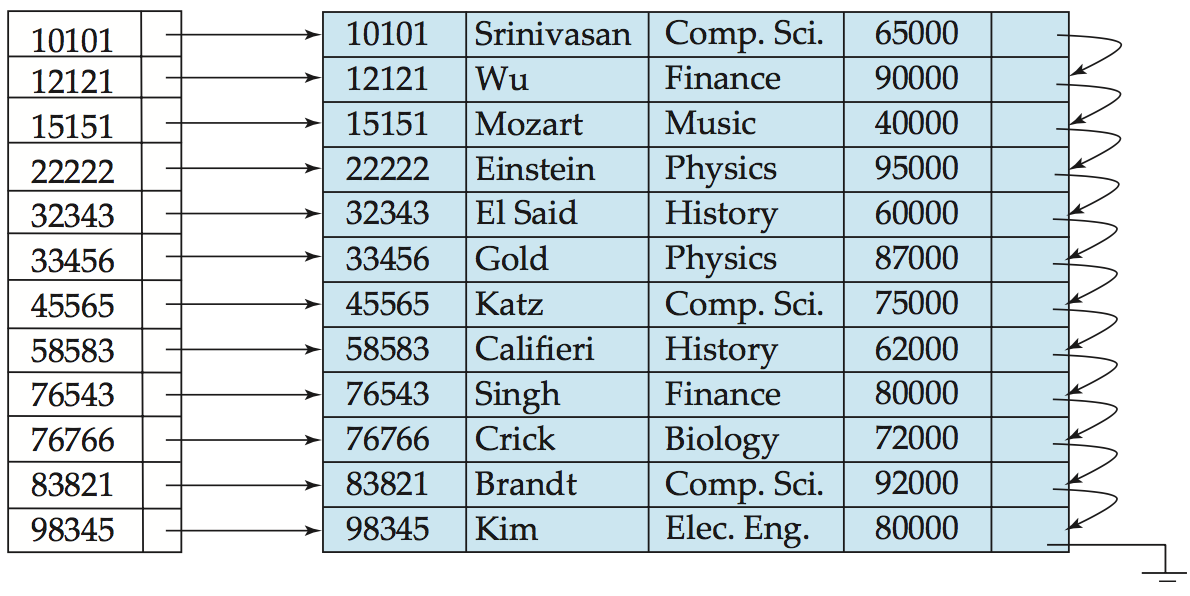
\includegraphics[width=0.49\textwidth]{images/dense-index}
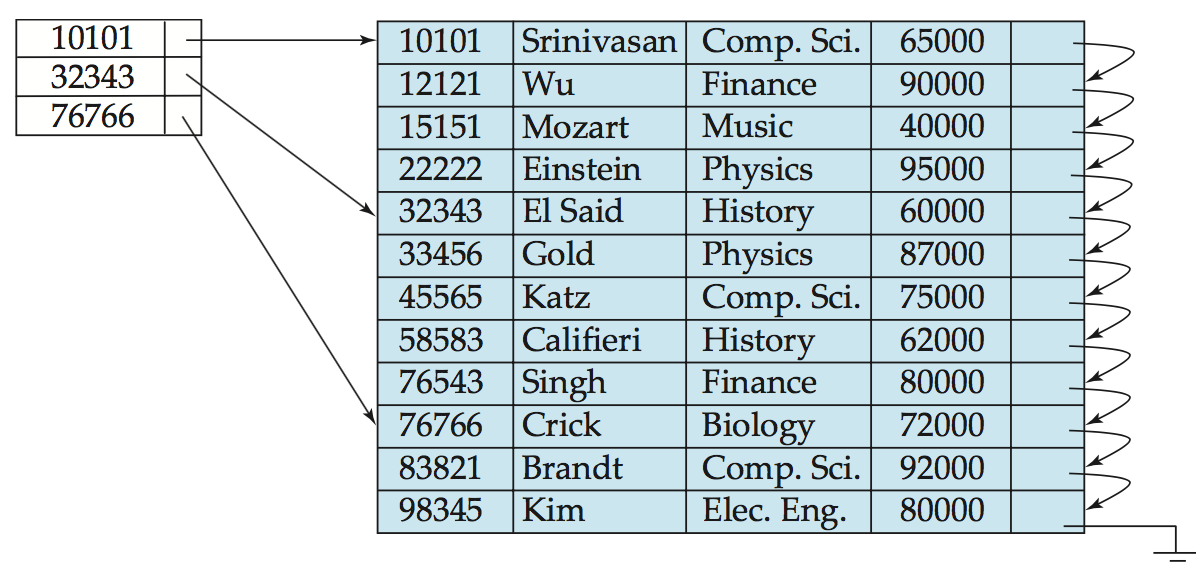
\includegraphics[width=0.49\textwidth]{images/sparse-index}
\end{center}


A small drawback to primary index has to do with re-ordering when insertion and deletion take place. 

\paragraph{Clustering Indexes.}
Suppose instead that records are ordered on a non-unique field. That means there is a clustering index and the clustering index is a lot like a sparse index. There is an entry for each of the distinct values of the ordering field. As a possible performance enhancement, to avoid the problem of insertion and deletion, one might have a block (or several) for each of the unique values of the ordering field~\cite{fds}.

As we generally discourage the use of non-unique fields in place of a primary index this scenario will not receive a great deal of attention.

\paragraph{Secondary Index.}

A secondary index, by definition, does not map to the order of the file. An index can be created on a unique field or a non-unique field and this, unlike clustering, is encouraged. As always, the index has two fields, the the indexing field and a block pointer (or record pointer). 

If a secondary index is on a unique field, there is one index for every record in the data file and the secondary index will be dense. We cannot leave things out, because the file is not ordered based on the attributes being sought. An example of what a secondary index would look like is shown below~\cite{fds}:

\begin{center}
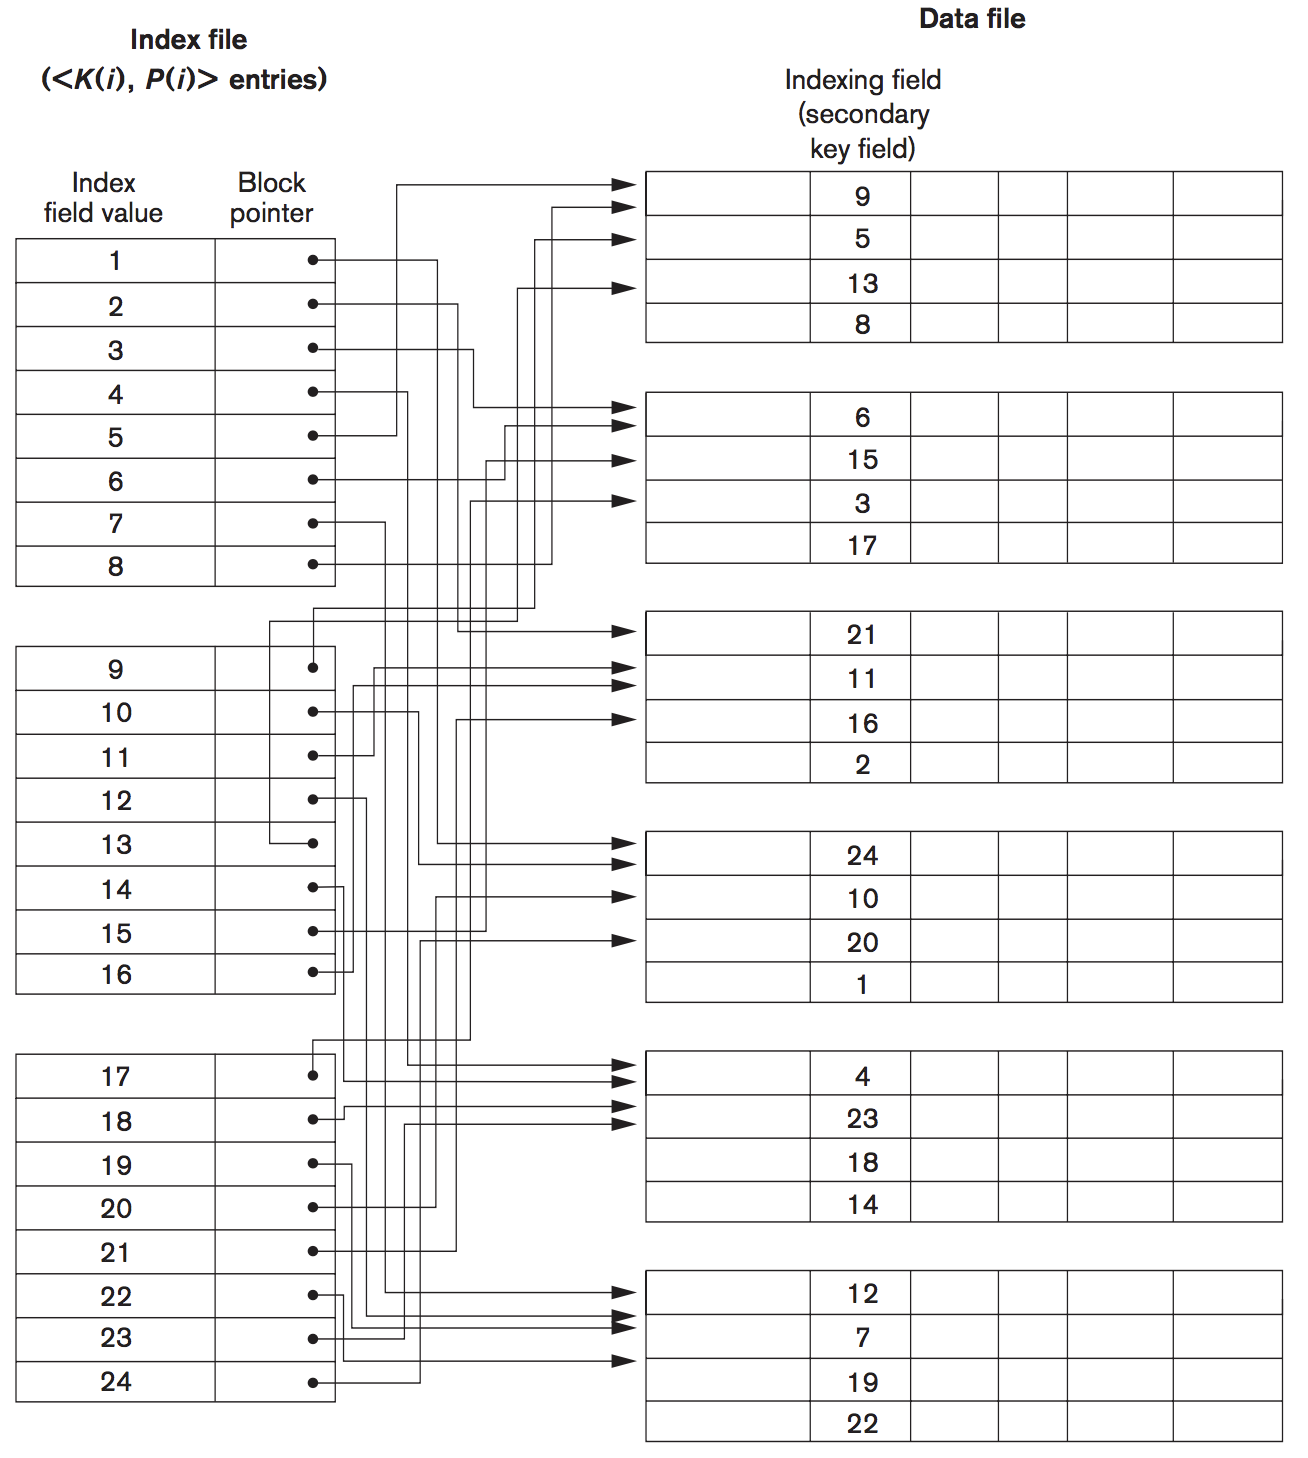
\includegraphics[width=0.8\textwidth]{images/secondary-index}
\end{center}

Of course, a secondary index does not have to be on a unique field. But that increases the complexity slightly. We could choose any one of these three options~\cite{fds}:

\begin{enumerate}
	\item \textbf{Duplicate entries} -- allow multiple index entries with the same value, maintaining a dense index. Our search routine must account for the fact that there could be multiple results with the same value. This would permit $<x, a>, <x, b>, <x, c>$ in the index.
	\item \textbf{Variable-Length Entries} -- entries can have variable length, so the tuple $<x, a>$ can now expand to be $<x, (a, b, c)>$. Again, the search algorithm must accept the fact that there are multiple elements on the right hand side.
	\item \textbf{Two-Level Index} -- There is an additional level of indirection so that the tuple references another block; this second block references the data blocks themselves.
\end{enumerate}

The two level index approach is very common. It is shown below in the diagram from~\cite{fds}: 

\begin{center}
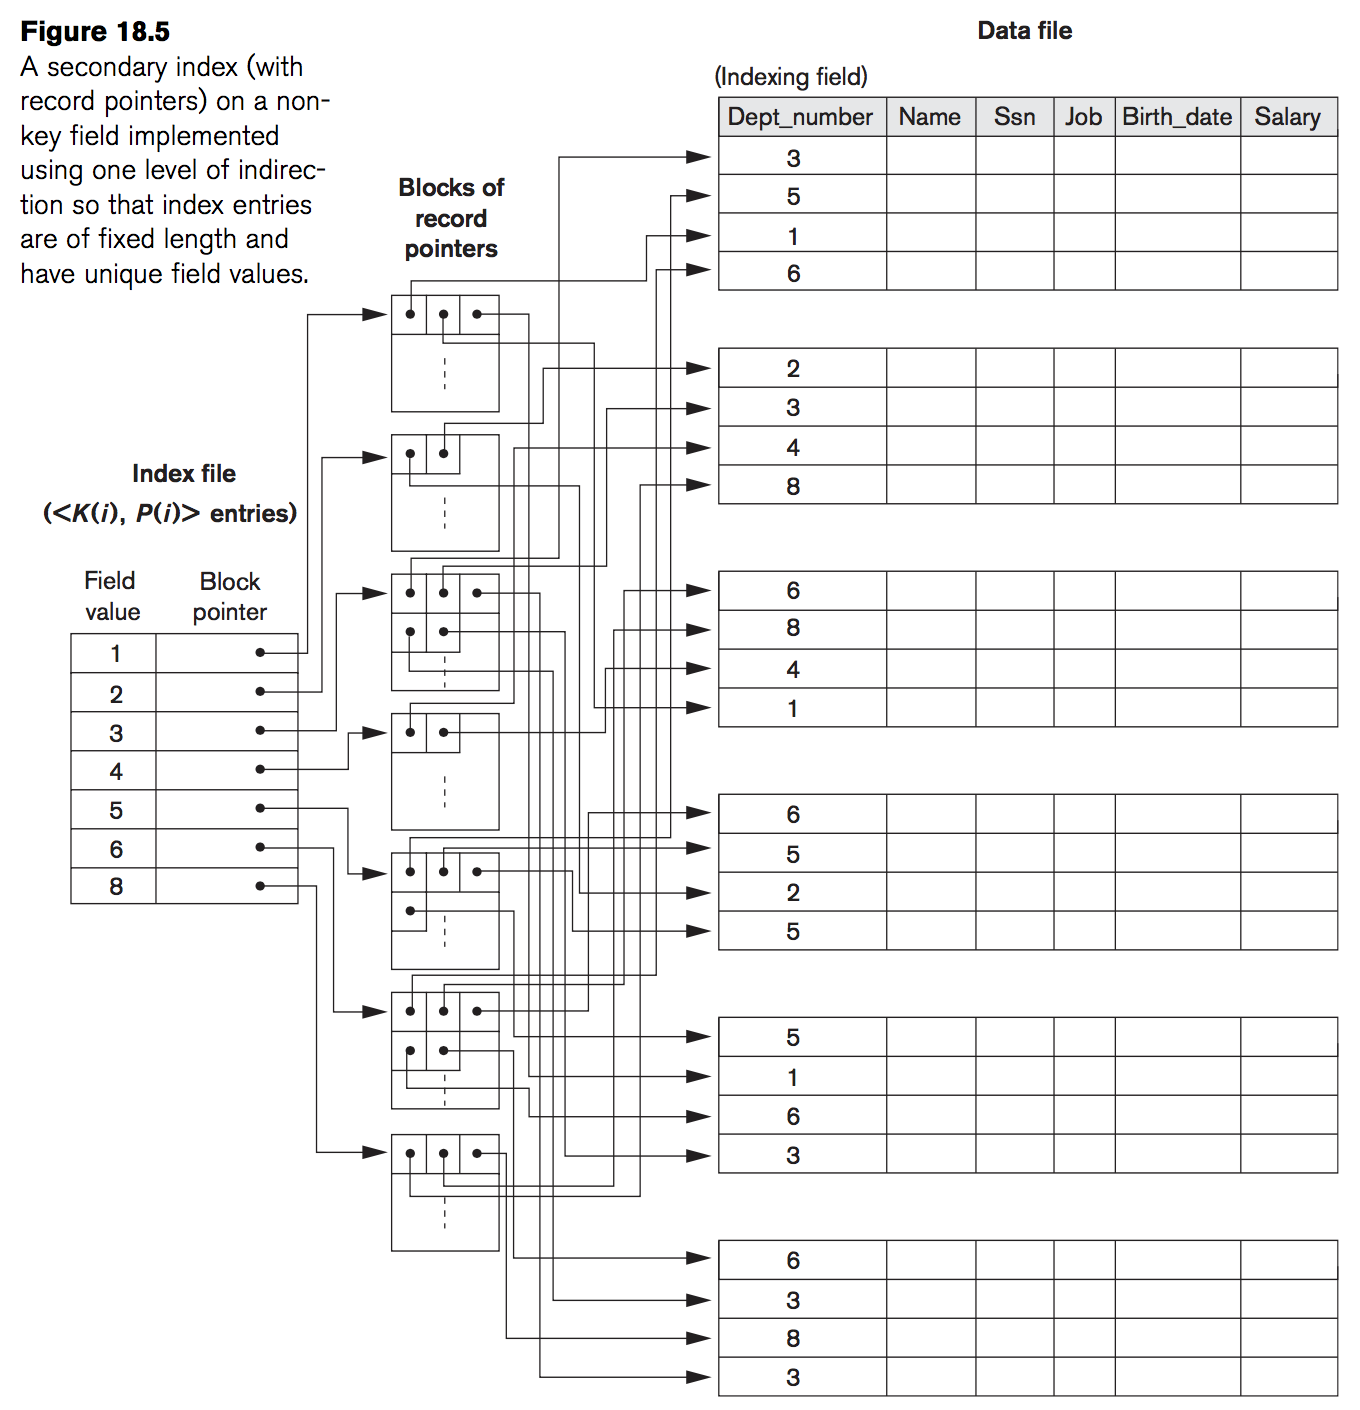
\includegraphics[width=0.85\textwidth]{images/secondary-index-2level}
\end{center}

Regardless of what implementation is used, operating on a secondary index is slower than operating on a primary index. That's okay, because it is still much better than not having an index at all, which would force linear searching. 

\paragraph{Next Steps.}
The secondary index has provided quick introduction to the idea of an index with multiple levels. The next topic will dig more into the subjects of multi-level indexing and the use of B+ Trees 

\subsection*{Updating an Index}

Regardless of the type of index, whenever a record is inserted or deleted, the index needs to be updated. If an update affects an indexed field, then it must also be updated. Calling back to updating a relation, an update can be modelled as a deletion and an insertion, which means we no longer need to consider update separately.

We will therefore consider two simple algorithms for insertion and deletion from~\cite{dsc}:

\paragraph{Insertion.}
If the index is dense, then:
\begin{enumerate}
	\item If the search key does not appear in the index, insert an index entry at the appropriate position.
	\item If the search key is found then:
		\begin{enumerate}
			\item If the index stores pointers to all records with the same search key value, add a pointer to the new record in the index entry.
			\item Otherwise the index entry stores a pointer to the first record with that value; place the record being inserted after the other records with the same key.
		\end{enumerate}
\end{enumerate}

If the index is sparse then:

\begin{enumerate}
	\item If a new block is created, insert the first search key value from the new block into the index.
	\item Otherwise, no new block is created and:
		\begin{enumerate}
			\item If the new record is the lowest record in the block, update the index entry for that block.
			\item If the new record is not the lowest, no change to the index occurs.
		\end{enumerate}
\end{enumerate}

\paragraph{Deletion.}

For deletion, the system must search to find the item to be deleted. If it's not there, of course, there's nothing to do. 

If the index is dense, then:
\begin{enumerate}
	\item If the deleted record was the only one with its value, delete that search key from the index.
	\item Otherwise:
		\begin{enumerate}
			\item If the index stores pointers to all records with the same search key value, delete the pointer to the deleted record.
			\item Otherwise: if the deleted record is the first in the group, update the pointer to be the next item; if it is not then there is no change to make.
		\end{enumerate}
\end{enumerate}

If the index is sparse then:

\begin{enumerate}
	\item If the index does not contain an entry with the deleted value, there is nothing to change.
	\item Otherwise:
		\begin{enumerate}
			\item If the deleted record is the only one with its search key, replace it with the next search key and record pointer; unless that is already in the index, in which case just delete the entry.
			\item If it is not the only one with its search key, then update the pointer to point to the next record with that same value.
		\end{enumerate}
\end{enumerate}

These algorithms are generally extensible to multi-level indexes as well: update the lowest level index and the changes will cascade upwards if needed. From the point of view of the second level, the lower level is the same as if it is a file containing records. But, as we will see, this is something we are about to examine.


\bibliographystyle{alphaurl}
\bibliography{356}


\end{document}
